%===================================================================================
% Chapter: Results
%===================================================================================
\chapter{Resultados}\label{chapter:results}
% \addcontentsline{toc}{chapter}{Análisis del conjunto de datos}
%===================================================================================

% introducción
Para iniciar la experimentación fue necesario normalizar los datos y luego se realizaron tres fases de experimentos. En la primera fase se probaron varias arquitecturas de red con el conjunto de datos original. Para la segunda fase se analizó la reducción de dimensiones utilizando el algoritmo de \'arboles aleatorios. Como ultima fase se modificó el conjunto de datos original para obtener uno nuevo y probar los algoritmos anteriores.

\section{Procesamiento de los datos}
% proceso de limpieza de datos
El conjunto de datos posee 42 características por cada entrada, las primeras 41 forman parte de la descripción del paquete de red y la última es la clasificación de este. Esta ultima puede variar, en los archivos con la extensión arff la clase es normal o anómalo, por otro lado, en los archivos txt, si el paquete es de un ataque, se especifica el tipo de ataque. Como se mencionó anteriormente, este documento se centra en la clasificación de los datos en normal y anómalos.

Para el proceso de normalización se investigaron todos los datos en los conjuntos de entrenamiento y de prueba. Las características de cada uno pueden ser de dos tipos, numéricas con valores reales o cualitativas con valores predefinidos. En el caso de las variables numéricas se escalaron todos sus valores al rango [0, 1] buscando el valor mínimo y máximo:
\[A_{i} = \frac{A_{i} - Min_{i}}{Max_{i} - Min_{i}}\] 
donde $i$ es la $i$-\'esima característica, $A_{i}$ es el vector de los valores de la característica de cada dato y $Min_{i}$, $Max_{i}$ son los valores mínimo y máximo de la característica respectivamente. Por otra parte, en las variables cualitativas se le asignó un índice a cada uno de los posibles valores comenzando por el 0, luego para escalarlos se dividió cada uno por la cantidad de posibles valores menos 1 para así obtener los datos en el rango [0, 1]:
\[A_{i} = \frac{index(A_{i})}{len(i) - 1}\]

\section{Modelos básicos}
% arquitecturas de redes simples con el dataset original
% 4x50                  CT-75.1  21T-52.76
% 64-128-64-32-16       CT-75.4  21T-53.25
% 64-128-128-64-32-16   CT-77.91 21T-58
Para un primer acercamiento al problema y para trazar una línea base superior al 50\% del algoritmo aleatorio se construyeron redes neuronales que entrenaron y se evaluaron con el conjunto de datos original. El modelo 1 posee una arquitectura de 4 capaz ocultas y cada una con 50 neuronas:
\begin{verbatim}
    from keras import models, layers

    model = models.Sequential()

    # Input - Layer
    model.add(layers.Dense(50, input_dim=(41), 
        activation='relu', name='input_layer'))

    # Hidden - Layers
    model.add(layers.Dropout(0.5))
    model.add(layers.Dense(50, activation='relu', 
        name='hidden_layer_1'))
    model.add(layers.Dropout(0.5))
    model.add(layers.Dense(50, activation='relu', 
        name='hidden_layer_2'))
    model.add(layers.Dropout(0.5))
    model.add(layers.Dense(50, activation='relu', 
        name='hidden_layer_3'))

    # Output - Layer
    model.add(layers.Dense(1, activation='sigmoid', 
        name='output_layer'))
\end{verbatim}

En este modelo, como en los restantes, se utilizó como función de activación en las capaz intermedias $relu$:
\[f(x)=max(0,x)\]
esta función es muy eficiente por si sencillez por lo que agiliza el proceso de entrenamiento. Por otra parte, en la capa de salida es necesaria la función $sigmoid$
\[f(x) = \frac{1}{1 + e^{-x}}\]
que tiene como resultado valores entre 0 y 1, dado que los datos de entrenamiento fueron modificados y los casos de tráfico anómalo tienen valor 1 y los normales valor 0 en su campo de clasificación, tomando los casos $< 0.5$ como tráfico normal y los $\geq 0.5$ tráfico anómalo

Este trabajo se centra en explorar los resultados de utilizar redes neuronales simples en el proceso de detección de intrusos, por lo que se analiza el comportamiento de los paquetes que viajan en la red por separado. Por lo antes mencionado, todos los modelos a probar utilizan capaz completamente conectadas o capaz densas como también se les conocen. La salida de estas capaz está representada por la siguiente función:
\[output = activation(dot(input, kernel) + bias)\]
donde $activation$ es la función de activación escogida, $dot$ es el producto punto entre dos vectores, $input$ es el vector con los valores de entrada, $kernel$ son los valores de peso de la red y $bias$ representa un valor de sesgo utilizado en los algoritmos de aprendizaje de máquina para optimizar los modelos.

Como en todos los casos se trabaja con redes neuronales de un tamaño considerable, varios ciclos de entrenamiento y un conjunto de datos con una gran cantidad de entradas, esto puede producir un sobreajuste en las fases de entrenamiento. Entre las técnicas de regulación m\'as usadas y efectivas se encuentra el \textit{dropout}. Solo se ejecuta en el proceso de entrenamiento y se aplica a las capas de la red. Consiste en la desactivaci\'on aleatoria de algunas de las características de salida de la capa en la que se encuentra, por ejemplo, si el factor de desactivaci\'on es de $0.5$ y la salida toma los valores [1, 0.7, 2.1,  0.3], se desactivan la mitad de las características y el resultado podría ser [1, 0, 0, 0.3]. Como medida de contención se le aplicó la técnica \textit{dropout} a varias capas intermedias de cada uno de los modelos.

En el proceso de entrenamiento llevado a cabo por cada modelo, se iteraron 100 veces sobre todos los datos(\textit{epochs}) en lotes de tamaño 64(\textit{batch}). Los resultados de la fase de entrenamiento del modelo 1 se pueden observar en la figura \ref{fig:4x5_train}. Para probar los modelos se utilizaron los dos conjuntos de datos de prueba expuestos en la sección \ref{section:dataset_description}. Como los resultados pueden variar con cada entrenamiento, se realizó este proceso 10 veces y se ejecutaron las pruebas en cada uno, obteniendo 10 resultados que se promediaron para tener un valor m\'as preciso.

\begin{figure}[t]
    \centering
    \subfigure{\label{fig:4x5_accuracy}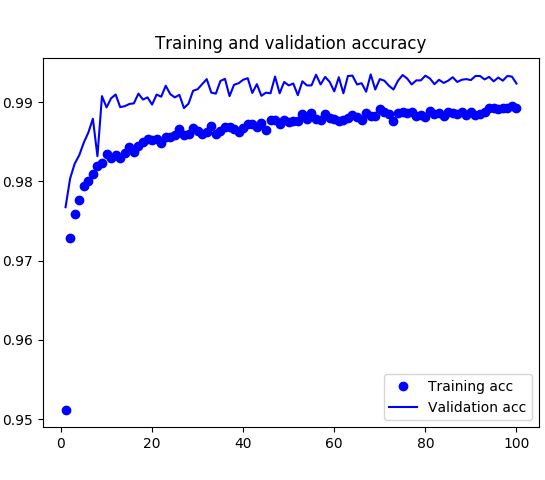
\includegraphics[width=.45\linewidth]{Images/4x50_accuracy.png}}
    \subfigure{\label{fig:4x5_loss}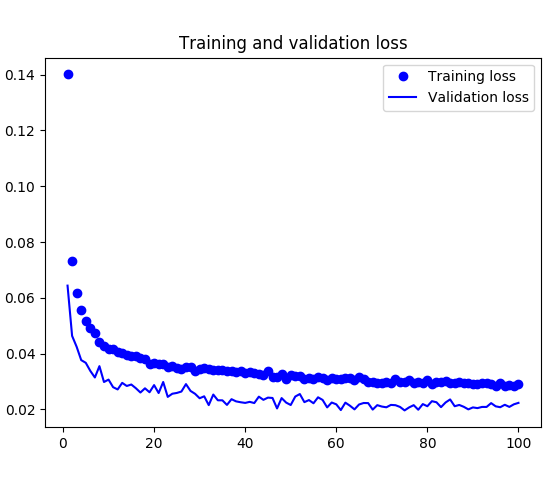
\includegraphics[width=.45\linewidth]{Images/4x50_loss.png}}

    \caption{Exactitud y pérdida en la fase de entrenamiento del modelo 1.}
    \label{fig:4x5_train}
\end{figure}

\begin{table}[b!]
    \begin{center}
        \caption{Resultados promedio del modelo 1 en los dos conjuntos de prueba.}

        \label{tab:model1_results}
        \begin{tabular}{c|c|c} % <-- Alignments: 1st column left, 2nd middle and 3rd right, with vertical lines in between
        \textbf{} & \textbf{KDDTest+} & \textbf{KDDTest-21}\\
        \hline
        Modelo 1 & 77.6392 & 57.5401\\
        \end{tabular}
    \end{center}
\end{table}

Se puede observar que los resultados obtenidos superan al 50\% del algoritmo aleatorio en ambos conjuntos de prueba. A pesar de ello los resultados obtenidos difieren de la fase de entrenamiento lo cual indica que el modelo no está generalizando correctamente los datos. En búsqueda de modelos con mayor comprensión de los datos se crearon dos nuevos, uno con 64, 128, 64, 32 y 16 neuronas en cada capa y el otro con 64, 128, 128, 64, 32 y 16 neuronas, en ese orden empezando por la primera capa oculta y terminando en la ultima respectivamente. Los comportamientos en las fases de entrenamiento fueron similares y los resultados se pueden observar en la tabla \ref{tab:model23_results}.

\begin{table}[t!]
    \begin{center}
        \caption{Resultados promedio del modelo 2 y 3 en los dos conjuntos de prueba.}

        \label{tab:model23_results}
        \begin{tabular}{c|c|c} % <-- Alignments: 1st column left, 2nd middle and 3rd right, with vertical lines in between
        \textbf{} & \textbf{KDDTest+} & \textbf{KDDTest-21}\\
        \hline
        Modelo 2 & 76.9894 & 56.2818\\
        Modelo 3 & 76.4411 & 55.2278\\
        \end{tabular}
    \end{center}
\end{table}

% TODO: poner la cita del chollet en el dropout, epochs y batch size
% TODO: explicar la función de optimizacion, la de perdida y las métricas

\section{Selección de características(incompleto)}
% selección de features
\begin{figure}[b]
    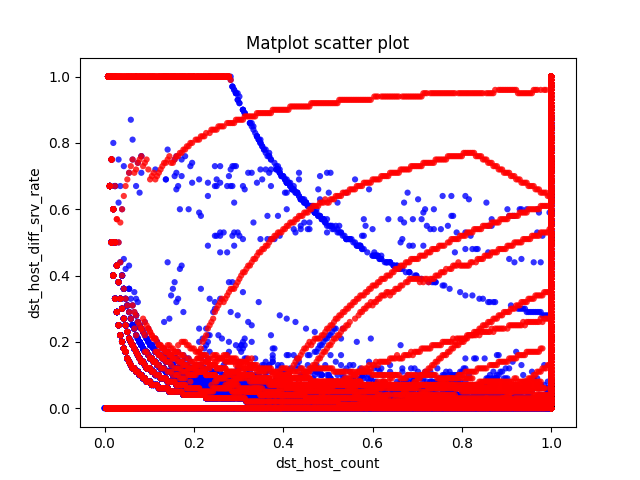
\includegraphics[width=\linewidth]{Images/dst_host_count-dst_host_diff_srv_rate.png}
    \caption{Gráfico que relaciona dos características de los datos. Los puntos rojos son anomalías y los azules tráfico común.}
    \label{fig:entropy}
\end{figure}

Para una mejor comprensión de los datos se realizaron multiples gráficas en las que se muestran una relación de dos de las características y datos de tráfico normal y anómalo. En la mayoría de estas existe una gran dispersión de los datos y no se observa un par de características evidentes que separen al conjunto como se puede observar en \ref{fig:entropy}. Por otra parte si se observan algunas que aportan muy poca o nada de información, esto se evidencia en \ref{fig:redundant}. En estos casos se tiene la característica $dst\_host\_diff\_srv\_rate$ que en la figura \ref{fig:entropy} si influye en la clasificación de los datos, sin embargo, en \ref{fig:redundant}, cualquiera sea el valor que tome los resultados no varían mucho.

\begin{figure}[t]
    \centering
    \subfigure{\label{fig:redundant_a}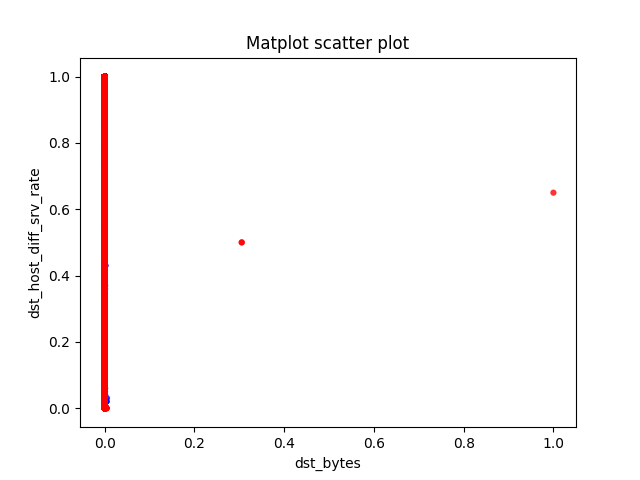
\includegraphics[width=.45\linewidth]{Images/dst_bytes-dst_host_diff_srv_rate.png}}
    \subfigure{\label{fig:redundant_b}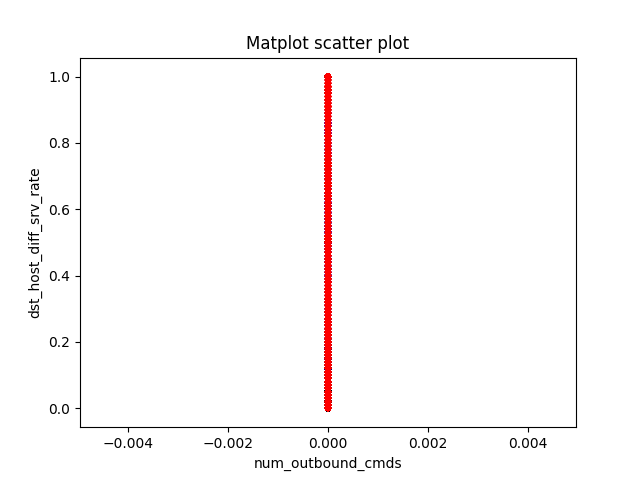
\includegraphics[width=.45\linewidth]{Images/num_outbound_cmds-dst_host_diff_srv_rate.png}}

    \caption{Característica innecesarias en los datos.}
    \label{fig:redundant}
\end{figure}

Las características redundantes hacen que a los modelos les tome más llevar a cabo la fase de entrenamiento o pueden causar un sobreajuste (\textit{overfitting}) que puede afectar la generalización, entre otros problemas\cite{tuv2009feature}.

Explicación y muestreo de resultados de la aplicación del algoritmo Random Forest para la extracción de las características de mayor importancia para la clasificación
% TODO: explicar la selección de parámetros para el random forest, poner las gráficas de la importancia de los features y mostrar resultados utilizando menos features.
% 30 features           CT-79.87 21T-61.85  76.79  55.90
% 64 batch size         CT-78.33 21T-58.82  77.07  56.43  77.13  56.53

\section{Transformación del conjunto de datos(terminar)}
% transformación del conjunto de datos
Unificación de los conjuntos de datos disjuntos del dataset original para la posterior creación de uno nuevo el cual contenga elementos de todas las dificultades

\subsection{Modificación del valor de aprendizaje(terminar)}
Variación del learning rate en el proceso de aprendizaje y búsqueda para el mejor resultado

\subsection{Validación por partes(terminar)}
Explicación del algoritmo de K-fold para una aproximación a un resultado mas real

% k-fold validation
% búsqueda del learning rate

% TODO: demostrar o probar porque con el dataset transformado no es necesario volver a probar los primeros modelos que eran mas malos con el dataset original